\documentclass[11pt,conference]{IEEEtran}
\IEEEoverridecommandlockouts
\usepackage{graphicx}
\usepackage{verbatim}
\usepackage{booktabs}
\begin{document}
\addtolength{\dbltextfloatsep}{-0.12in}
\addtolength{\textfloatsep}{-0.12in}
\title{Exploring causal factors affecting recycling efficiency in England}
\author{
Justin Salmon, George Lancaster, \\Xiangtian Zheng, Srijan Chhabda, Nelly Deprince\\
{\normalsize \{wr18313,qv18258,io18763,ev18326,nd15823\}@bristol.ac.uk}\\
\\https://github.com/jlsalmon/comsm0017}
\maketitle
\begin{abstract}
Domestic waste production remains one of the most gravely serious problems facing humanity in the 21st century, despite global efforts to improve recycling rates. This project aims to apply data science techniques to fuse historical recycling rate data in England with multiple other data sources, in a search for potentially indicative factors that could be used to predict future recycling rates. Despite none of the investigated factors being found to be meaningfully correlated, a number of predictive regression models were evaluated and found to give reasonably accurate predictions.
\end{abstract}

\section{Introduction}
The amount of waste produced globally is staggering. In England alone, there are around 40 million tonnes of household waste generated every year, of which around 18 million is recycled \cite{Defra2019}, giving England a recycling efficiency score of around 40-45\% (depending on which types of waste are included in the calculations). England is far behind other countries in Europe such as Switzerland and the Netherlands, which recycle around 60\% of their total waste.

It is not difficult to find some horrendous facts and statistics about recycling. For example, an entire rubbish truck worth of plastic is dumped into the ocean every single minute \cite{Pennington2016}. It is estimated that by 2050, there will be more plastic in the ocean by weight than fish \cite{Connor2016}. Clearly these facts are shocking to learn, and are the main motivation behind this research. As a society, we urgently need to improve our recycling behaviour to prevent irreversible damage to our planet.

Our task with this project is to try to use data science and machine learning techniques on historical recycling data in England, along with a number of other data sources, to try to identify causal factors that affect household recycling behaviour. If these factors can be found, they can potentially be used to predict future recycling rates. Furthermore, they can potentially be used to influence the policies of the authorities in charge of recycling infrastructure. 

\textbf{Aims}: This project aims to identify causal factors that can be used to accurately predict future recycling rates. 

\textbf{Objectives}: In order to achieve that aim, a variety of statistical analysis and machine learning techniques will be applied to historical English recycling data along with additional data from a number of sources.

If successful, our findings can potentially be used by local authorities to inform their waste management policies and promote positive change in recycling behaviour.

\begin{figure*}[h]
\begin{center}
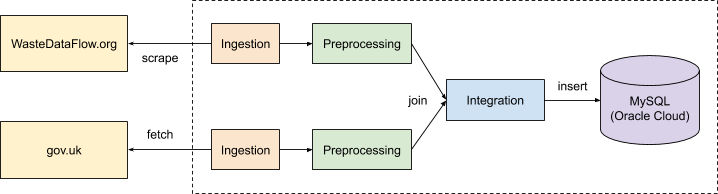
\includegraphics[width=\linewidth]{figures/architecture.png}
\caption{Data ingress pipeline architecture}
\label{fig:architecture}
\end{center}
\end{figure*}
\section{Obtaining Data}
In order to be able to make predictions about future recycling rates, it is of course necessary to obtain historical recycling data, and also data which may contain potentially causal variables over the same time period. This section describes the data sources that were used, as well as the pipeline that was built by which the data was ingested and prepared for use. Data was obtained from two primary sources: the WasteDataFlow portal and the UK Government data portal.

Figure \ref{fig:architecture} shows an overview of the architecture of the data ingress pipeline developed in this project. The following subsections will describe each section of the pipeline in turn.
\subsection{WasteDataFlow}
The UK Environment Agency publishes annual waste figures dating back to 2006 for each local authority, as summary spreadsheets in Excel format \cite{UKGovernment2018}. However, the format and quality of these summary spreadsheets is inconsistent year-on-year, with some years being absent entirely. Due to this, the decision was made to instead extract and manually process raw data from the WasteDataFlow portal, which is the original source of the summary data. 

WasteDataFlow \cite{WasteDataFlow} is the central system used by all local authorities in the UK to report waste statistics to government. Local authorities are required to input values for a number of predefined fields such as total amount of kerbside household black-bag, recycling and garden waste collected (measured in tonnes) and their final destinations (landfill, incineration, recycling plants, export, etc.).
\subsubsection{Ingress}
WasteDataFlow unfortunately does not expose a programmatic API. In order to extract data, a web-based export tool must be used. The user must select the desired time ranges and authorities, as well as selecting the specific fields that are to be included in the export. The export produces a zipped Excel spreadsheet containing the requested data. To facilitate this process and create a reproducible ingestion pipeline, an automated web scraper was built using the \texttt{selenium} library which automatically exports data from WasteDataFlow. Data was exported for all available years (2006-2017) for each local authority in England. All available fields were included in the export in order to allow selection of appropriate fields further downstream in the pipeline. The web scraper loads the exported Excel spreadsheet into a \texttt{pandas} dataframe and hands it over to the preprocessor.
\subsubsection{Preprocessing}
The WasteDataFlow export format is highly non-normalised and quite esoteric, with each field name existing as a row under the heading “RowText” and its corresponding data value as a row under the heading “Data”. As such, in order to wrangle it into a useful format, it is necessary to perform a \textit{pivot} on the dataframe to transform the “RowText” rows into column headers and the “Data” rows into values underneath their respective headers. At this point, unwanted columns and rows are removed, NaN values are set to zero, and number-like string values are converted to proper numeric values. Since WasteDataFlow reports quarterly, the data values are aggregated to an annual figure based on an appropriate aggregation function (e.g. \texttt{sum} for recycling tonnage and \texttt{avg} for recycling efficiency).

A major step in the preprocessing stage is to handle the many changes to local authority government structure that have happened since 2006. Throughout that time, many authorities have been abolished and merged into other authorities, and many new authorities have been created. This presents a challenge to accurately track historical figures without accidentally duplicating or omitting data. 

Our approach to this problem was to obtain an official list of local authorities for the most recent year (2017) and use it as a reference point. Data for previous years is then “coalesced” to the reference list. For example, in 2009, the six Cornish districts of "Penwith", "Kerrier", "Carrick", "Restormel", "Caradon" and  "North Cornwall" were combined into the single “unitary authority” of “Cornwall”. Thus, for pre-2009 data, these six districts are aggregated into a synthesised “Cornwall” authority to match the 2017 reference. Similar aggregations or disaggregations are performed for all other structural changes, until data for each year contains the same set of authorities. Assertions are added to the code to ensure the correct authorities are present. This results in much simpler downstream code, and does not significantly affect results.

\begin{figure*}[htbp]
    \begin{center}
        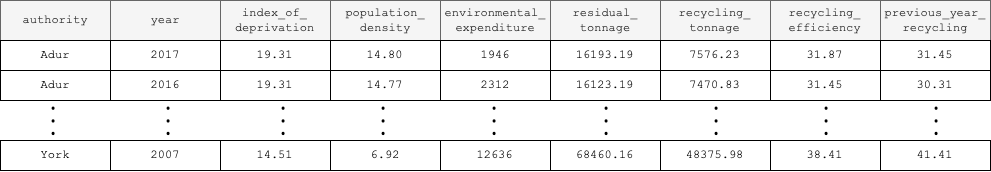
\includegraphics[width=\linewidth]{figures/db_structure.png}
    \caption{Structure of the database table}
    \label{fig:db_structure}
    \end{center}
\end{figure*}

\subsection{UK Government}
The UK Government publishes annual expenditure reports for each local authority \cite{UKGovernment2019}. These reports contain breakdowns of how authorities have distributed their budgets over a number of categories such as education, policing and fire services, healthcare and environmental services. A number of other annual metrics are also available from the Government portal in separate reports, which include properties such as estimates for total population, population density and “index of deprivation” \cite{ocsi}. The combination of these properties will form the basis of our correlation and predictive analysis later on in this report.
\subsubsection{Ingress}
The Government portal data exists as a set of links to downloadable Excel spreadsheets only, and does not provide a programmatic API. In order to have an automated ingress stage, a simple script was developed to fetch the spreadsheets by URL via HTTP. They are then loaded into a \texttt{pandas} dataframe and passed to the preprocessor.
\subsubsection{Preprocessing}
The Excel spreadsheets are unfortunately not in a particularly consistent format. Sheet names, column names and general layout (such as header/footer locations) all differ year-on-year. This resulted in some slightly unattractive code to wrangle each year to make it consistent. Following that, unwanted rows and columns were dropped, NaN values set to zero, and number-like string values converted to proper numeric values.

Using the same strategy as for the WasteDataFlow data, the local authorities are coalesced to match the reference list for 2017. Thankfully we were able to reuse the same code to achieve this. Assertions were added to ensure the list matches the reference for each year.
\subsection{Integration and Storage}
Once the two data sources are ingested and preprocessed, they are then integrated into a single \texttt{pandas} dataframe. Since the preprocessing stage ensures consistency of local authority names, the integration is a simple join on local authority name and year columns.


The preprocessed data was placed into an SQL database table. While the data could have been stored as CSV or Excel files, using an SQL database allows all team members to access the data in a uniform way. It also drastically speeds up the process of analysing and visualising the data, since performing an SQL query is about two orders of magnitude faster than running the entire ingestion/transformation pipeline.

The structure of the database table is shown in Figure \ref{fig:db_structure}, containing all properties that were extracted from both data sources. The \texttt{authority} and \texttt{year} columns comprise the composite primary key and primary index of the table. Since each additional property is relevant only to a specific authority/year key pair, it is sufficient to simply include them as columns. Using multiple tables is not necessary in this case. The entire combined dataset for all available years contains 4404 rows, and has a fairly small size of 48MB. The database itself is a MySQL instance hosted in the Oracle cloud.

\subsection{Ethics and privacy}
As far as we are aware, there are no direct privacy concerns with any of the data sources used in this research, since there is no personally identifiable information contained within them. We also do not believe there to be any relevant ethical issues with this study.
\section{Exploratory analysis}
In order to understand its basic characteristics, we performed some exploratory analysis on our data. We initially wanted to find out which regions are better or worse at recycling, and how recycling behaviour has changed throughout the period under study.

Figure \ref{fig:hist_rec_eff} shows the average recycling efficiency (measured as a percentage of total waste collected) for all local authorities from 2006 to 2017. It is clear that there is has been a steady improvement in efficiency since 2006, although this levels off around 2012 and even begins to drop slightly in 2014. It is not known why this is the case, although there appear to be several theories. For example, some argue that England is suffering from “green fatigue”, whereby people are losing motivation to recycle due to the extra effort, and possibly due to certain media sources questionably reporting that recycling isn’t as effective as it is claimed to be \cite{gosden_2014}. Whatever the true reason(s), this finding further motivates us to find out what can potentially be done to improve the situation.

\begin{figure}[htbp]
    \begin{center}
        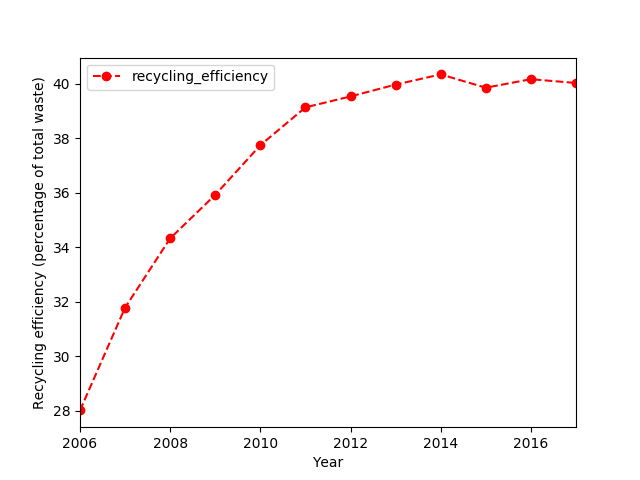
\includegraphics[width=\linewidth]{../figures/england_historical_recycling_efficiency.png}
    \caption{Historical recycling efficiency, 2006-2017}
    \label{fig:hist_rec_eff}
    \end{center}
\end{figure}

Figures \ref{fig:heatmap2006} and \ref{fig:heatmap2016} show heatmaps of recycling efficiency in England for both 2006 and 2017, which allow us to succinctly observe how efficiency differs throughout the country. The overall improvement in efficiency can clearly be seen from the darker blue nature of the 2017 plot. It appears that in 2006, the Midlands were generally the most efficient recyclers, whereas London, the North and the Westcountry were lagging slightly behind. By 2017, efficiency became more uniformly distributed overall. However, the North and London are still noticeably less efficient. The reason for the observed regional disparity is not obvious, although it is hypothesised that population density and relative wealth may have an effect. We will investigate these hypotheses further throughout this report.

In addition to these static heatmaps, a web-based interactive version was also developed using Leaflet.js, backed by a REST API deployed to the Oracle cloud. The API connects to our database and provides data for the frontend web interface. The interactivity provided by this web-based version facilitates quick inspection of exact recycling rates for individual regions.

\begin{figure}
    \centering
    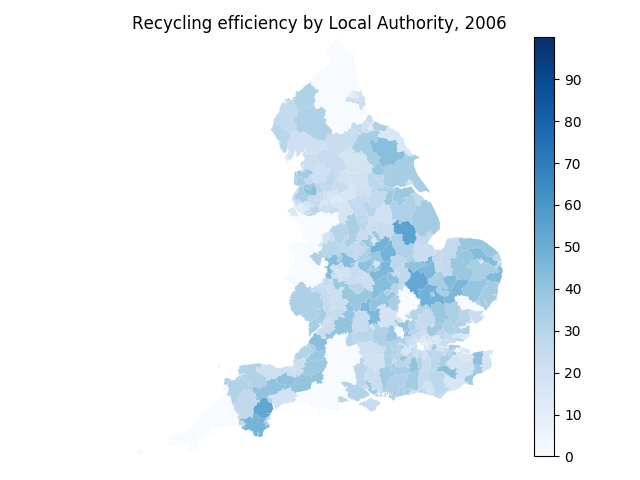
\includegraphics[width=\linewidth]{../figures/england_recycling_heatmap_efficiency2006.png}
    \caption{Recycling efficiency heatmap for 2006}
    \label{fig:heatmap2006}
\end{figure}

\begin{figure}
    \centering
    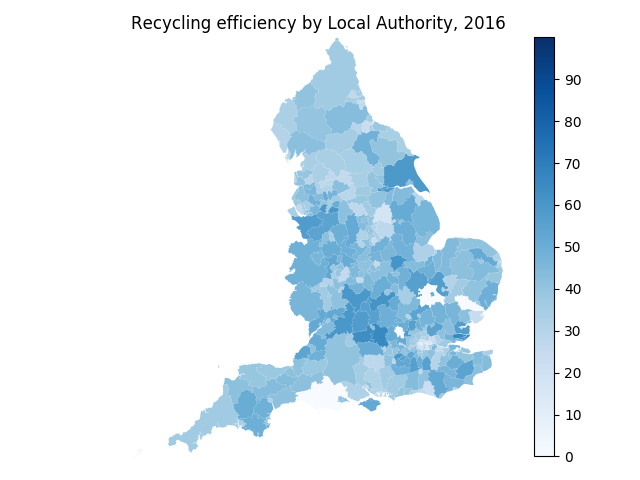
\includegraphics[width=\linewidth]{../figures/england_recycling_heatmap_efficiency2016.png}
    \caption{Recycling efficiency heatmap for 2016}
    \label{fig:heatmap2016}
\end{figure}



To give us another view on which local authorities have made the most (and least) improvements since 2006, we decided to create an “improvement rankings” plot, as seen in Figure \ref{fig:rec_improvement_rankings}. This shows the difference in recycling efficiency between 2006 and 2017. It can be seen that about the vast majority of authorities have made improvements, with some notable successes such as Rochford, Stroud and Ashford. However, there are a number of authorities which have gotten worse, with Forest Heath being the worst offender at about -13\% efficiency since 2006. On average, the efficiency improvement is about 12\%, which corroborates with Figure \ref{fig:hist_rec_eff}. It is known that the Government has a national target of 50\% recycling efficiency by 2020, so it is encouraging to see that some authorities are heading toward that target. However, the majority of authorities are well below the target.


\begin{figure*}[htbp]
    \begin{center}
        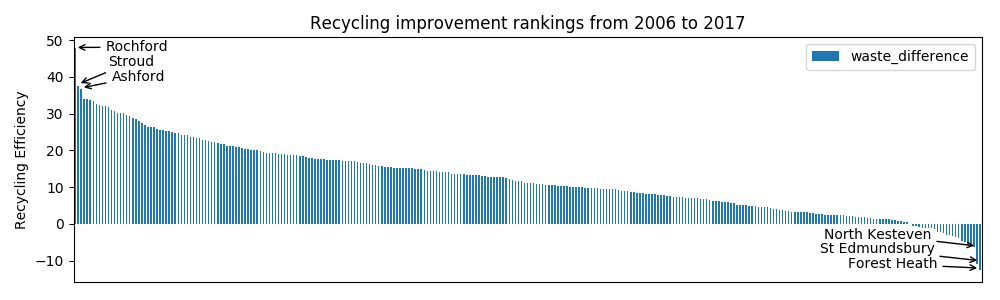
\includegraphics[width=\linewidth]{../figures/england_historical_recycling_improvement_rankings.png}
    \caption{Recycling improvement rankings from 2006 to 2017}
    \label{fig:rec_improvement_rankings}
    \end{center}
\end{figure*}

\section{Correlation measures}
Following our initial exploratory analysis, we moved on to attempting to identify correlations between recycling efficiency and a number of potentially causal variables that we collected from the UK Government data portal as well as the WasteDataFlow system. The Pearson and Spearman correlation coefficients were used to determine the relationship between our explanatory variables and response variables. The Pearson correlation coefficient allows us to quantify any linear correlations, and Spearman allows us to quantify any monotonic correlations in our data. Correlation does not always mean that there is causative relationship between variables, however it can help to identify variables of interest. 
\subsection{Pearson correlation coefficient (PCC)}
The PCC is defined as the measure of linear correlation between two variables $X$ and $Y$ \cite{ROUSSEAU201867}. It results in a correlation coefficient $\rho$ in the range -1 to +1 where +1 is a perfect positive linear correlation and -1 is a perfect negative linear correlation. Values greater than 0.8 are generally considered to be significant, however this is dependent on the problem domain. Linear correlations can be very informative, and can also be indicative of a causal relationship. It is therefore important to determine if there are any linear correlations in our data. Pearson correlation requires that the data is normally distributed and scaled to values between 0 and 1.  It is formally expressed in Equation \ref{equation:pcc}.

\begin{equation}
\rho = \frac{cov(X,Y)}{\sigma_{X}\sigma_{Y}}
\label{equation:pcc}
\end{equation}

Where $cov$ is the covariance, $\sigma_{X}$ is the standard deviation of $X$ and $\sigma_{Y}$ is the standard deviation of $Y$.

\subsection{Spearman correlation coefficient (SCC)}
The Spearman Correlation Coefficient (SCC) is defined as the ‘Pearson correlation coefficient between the rank variables’ \cite{ROUSSEAU201867}, and it is used to assess monotonic relationships between two variables. Similarly to Pearson correlation, it results in a correlation coefficient $\rho$ in the range -1 to +1, where +1 is a perfect Spearman correlation. Monotonic relationships can also indicate causal relationships, and establishing if these exist is a key parts of data analysis. Spearman correlation is formally expressed in Equation \ref{equation:scc}.

\begin{equation}
r _ { s } = \rho _ { \mathrm { rg } _ { X } , \mathrm { rgy } } = \frac { cov  \left( \mathrm { rg } _ { X } , \mathrm { rg } _ { Y } \right) } { \sigma _ { \mathrm { rg } _ { X } } \sigma _ { \mathrm { rg } _ { Y } } }
\label{equation:scc}
\end{equation}

Where $\rho$ is the pearson correlation of the rank variables, $cov(rg_{X}, rg_{Y})$ is the covariance of the rank variables, and $\sigma_{rg_{X}}$ and $\sigma_{rg_{Y}}$ are the standard deviation of the rank variables.

\begin{table*}[!ht]
\centering
\caption{Pearson and Spearman correlation coefficients for each explanatory variable and response variable.}
\begin{tabular}{@{\extracolsep{4pt}}ccccc}
\toprule
& \multicolumn{2}{c}{\textbf{Recycling quantity}} & \multicolumn{2}{c}{\textbf{Recycling efficiency}}\\
\cmidrule(lr){2-3} \cmidrule(lr){4-5}
\textbf{Explanatory Variable}       	& \textbf{PCC} $\rho$ & \textbf{SCC} $\rho$ & \textbf{PCC} $\rho$ & \textbf{SCC} $\rho$   \\
\midrule
environmental\_expenditure         			 & 0.717           	& 0.717 & -0.381           	& -0.314              	\\
environmental\_expenditure\_adjusted   	 & -0.252          	& -0.642  & -0.218          	& -0.291             	\\
population                          	& 0.839           	& 0.826     	& -0.224           	& -0.216      	\\
population density                  	& 0.119           	& 0.284 	& -0.385           	& -0.416        	\\
Index of deprivation                	& 0.258           	& 0.227	& -0.454           	& -0.464         	\\
\bottomrule
\end{tabular}
\label{table:quantity}
\end{table*}
\subsection{Variables}
Other studies suggest that public attitude and ecological involvement are the biggest factors that contribute towards recycling behaviour \cite{Valle2005, nishio_chizuru_takeuchi_toshie_1970}. Our focus is on finding other variables that have a causal relationship with domestic recycling from governmental budgets and demographic data.
\subsubsection{Explanatory Variables}
Explanatory variables are suspected of being independent, however this cannot be known for certain. All explanatory variables used in this study are given per local authority and are summarised in the following list:

\begin{itemize}
\item $environmental\_expenditure$: The amount of money spent on environmental services in GBP (£);
\item $environmental\_expenditure\_adjusted$: The amount of money spent on environmental services per person (£ / person);
\item $population$: Total number of people residing in a local authority jurisdiction;
\item $population\_density$: The number of people residing in each unit of area governed by the authority;
\item $index\_of\_deprivation$: A relative measure of poverty, areas with a higher score are more deprived;
\item $previous\_year\_recycling$: The recycling efficiency of a local authority for the previous year. 
\end{itemize}


Environmental services is a blanket term that encompasses a wide range of services including recycling, waste disposal, pest control, water safety and food safety, amongst other things. Therefore it may not accurately reflect the amount of money spent on recycling services alone. Unfortunately is was not possible to obtain fine-grained breakdowns of environmental spending.

\subsubsection{Response Variables}
We aim to map a relationship between the explanatory variables and the response variable, whereby the response variable is dependent on the explanatory variables. We have performed analyses on two response variables:

\begin{itemize}
\item $recycling\_quantity$: the total recycling per local authority (Tonnes);
\item $recycling\_efficiency$: the percentage of total recycled waste per local authority (\%).
\end{itemize}

\subsection{Discussion}
It can be expected that population will influence the total quantity of recycling generated by a local authority. To account for this, we calculate the recycling efficiency using Equation \ref{equation:efficiency}

\begin{equation}
re = \frac{recycling\_quantity}{(residual\_waste + recycling\_quantity) \cdot 100}
\label{equation:efficiency}
\end{equation}

which gives the percentage of total waste that is recycled for each authority.

Table \ref{table:quantity} shows that there is a significant correlation between environmental expenditure and total recycling quantity. However, there is no correlation once adjusting for the population, suggesting that the $population$ variable is confounding, and is the root cause of the correlation. Local authorities that govern a larger population can be expected to have a bigger budget and will therefore spend more on environmental services. To account for this, we introduced the $environmental\_expenditure\_adjusted$ variable, which is calculated using Equation \ref{equation:adjusted}.

\begin{equation}
eea =\frac{environmental\_expenditure}{population}
\label{equation:adjusted}
\end{equation}

This describes the amount of money spent on environmental services per person for each local authority. Testing for correlation using this variable results in no significant correlation using either Pearson or Spearman tests, suggesting that there is no linear or monotonic relationship between these variables.

\begin{table*}[!ht]
\centering
\caption{Results of the regression analysis. Each variable was tested on each regression model and on all possible combinations of variables. The final row shows each model when trained using the index of deprivation, population density, and previous years recycling efficiency.}
\begin{tabular}{@{\extracolsep{1pt}}cccc}
\toprule
   					 &    \textbf{Multiple Linear Regression}    & \textbf{Random Forest}   	 &    \textbf{Neural Network}  \\
\cmidrule(lr){2-2} \cmidrule(lr){3-3} \cmidrule(lr){4-4}
\textbf{Explanatory Variable}  &   \multicolumn{3}{c}{$\mathbf{R^2}$ \textbackslash \textbf{RMSE}}. \\
\midrule
   					 
Previous year recycling (a)  		 & 0.932  \textbackslash 2.638 	& 0.935 \textbackslash 2.591   & 0.947 \textbackslash 2.331                       	\\
Environmental expenditure adjusted (b) & -0.011 \textbackslash 10.184   & -0.299 \textbackslash 11.542& 0.004 \textbackslash 10.107                    	\\
Index of deprivation (c)                		 & 0.291  \textbackslash 8.521 	& 0.823 \textbackslash 4.264   & 0.321 \textbackslash 8.343                      	\\
Population density   (d)           			 & 0.235 \textbackslash 8.856  	& -0.104 \textbackslash 10.638& 0.293 \textbackslash 8.515                      	\\
\midrule
(a), (c), (d) &0.935 \textbackslash 2.583 & 0.935 \textbackslash 2.575 &0.947 \textbackslash 2.323 \\
\bottomrule
\end{tabular}
\label{table:params}
\end{table*}

Pearson and Spearman correlation coefficients have similar limitations, and are limited to measuring only linear or monotonic relationships respectively. Therefore significant correlations may exist even if both tests result in a coefficient of 0. Additionally, neither test can measure the temporal qualities of the data. A change to environmental spending may not affect recycling rates until many years later when the benefit of the increased spending is realised. As our data is historical, and changes over time, we propose another explanatory variable $previous\_year\_recycling$, which is the recycling efficiency of a local authority for the previous year.

\subsection{Hypothesis}
We hypothesise that there is a nonlinear relationship between the explanatory variables and recycling efficiency that is unmeasurable using a correlation coefficient or through visual inspection. We have performed a number of regression analyses to test this hypothesis. If a variable can be used to make a prediction on future recycling efficiency, we can assume that a regression model has learned a relationship undetectable through correlation alone.

\section{Regression Models}
To make predictions about future recycling efficiency, we used three machine learning models to perform a regression analysis. To do this, we used the set of explanatory variables from Table \ref{table:params}, coupled with recycling efficiency for the previous year, as the inputs to our models. The three models used were a multiple linear regression model, a random forest model and a three-layered neural network.
\subsection{Multiple linear regression}
A multiple linear regression model aims to map the relationship between two or more explanatory variables and a response variable by fitting a linear equation to the observed data \cite{kenton_2019}. One of the problems with this method is that it assumes that the relationship between the explanatory variables and the response variable are linear, which appears not to be the case for our data.

Multiple linear regression is formally described using Equation \ref{equation:linearregression}
\begin{equation}
y_{ i } = \beta_{ 0 } + \beta_{ 1 } x _ { i 1 } + \beta _ { 2 } x _ { i 2 } + \ldots + \beta _ { p } x _ { i p } + \epsilon
\label{equation:linearregression}
\end{equation}

where, for $i=n$ observations, $y_{i}$ is the response variable, $x_i$ is the explanatory variable, $\beta_0$ is the $y$ intercept, $\beta_p$ is the slope coefficients for each explanatory variable and $\epsilon$ is the error term.

\subsection{Random forest regression model}
A random forest is an ensemble of decision trees. It uses a training method known as `bootstrap aggregating’, which involves splitting the training data $X=\{x_{1},...,x_{n}\}$, and training targets $Y=\{y_{1},...,y_{n}\}$ into sub-samples with each tree $t$ in the ensemble trained on a single data sample. Each sample is taken using a random sample with replacement approach, which means that data can be reused for more than one decision tree. To make a prediction, the output from a random forest is the mean value given across all decision trees in the ensemble.

\subsection{Neural network regression}
We used the \texttt{keras} wrapper around the \texttt{tensorflow} library to create a three-layered neural network. Neural networks are typically used for classification problems, however they can be used for regression tasks by using a linear activation function in the final layer. Our neural network is trained for 200 epochs, but only saves the weights when the validation mean absolute error is at its lowest. This ensures that we get the best possible model from the training run, whilst avoiding overfitting.

When training, we used a validation split of 0.15. This takes 15\% of the training data and uses it to validate the model at each training epoch. This data is always unseen, and is only used to the measure the performance of the model. It is typically used to indicate overfitting if the training accuracy is high, but the validation accuracy is low. We have chosen to minimise the mean absolute error during optimisation, which is the measure of difference between the predicted value and the true value. This is a negatively oriented score, meaning that a lower values indicates a better performance. 

\section{Hyperparameter Tuning and Model Evaluation}
Hyperparameters are defined as parameters whose values are set before the learning process begins \cite{agrawal_agrawal_2019}. They are external to the model, and cannot be learned from training data. Setting values for such parameters is non-trivial, and can done using a brute-force approach known as \textit{gridsearch}.

Gridsearch performs a parameter sweep across all possible combinations of a predefined set of parameter configurations. For each configuration, a model is trained and evaluated. Given a large set of parameters, this process can be highly computationally demanding \cite{lerman1980fitting}. To achieve the best possible results, it is often coupled with \textit{K-fold cross-validation}. This is resampling procedure that enables model evaluation on a limited amount of data. It splits a data set into $k$ equally sized samples, with $k-1$ training samples, and 1 sample reserved for validation. This process is repeated $k$ times, with each sample used as the validation sample only once. The average score across all iterations is used to judge the performance of the model. This process is visualised in Figure \ref{fig:five_fold_cv}.

\begin{figure}[htbp]
	\begin{center}
    	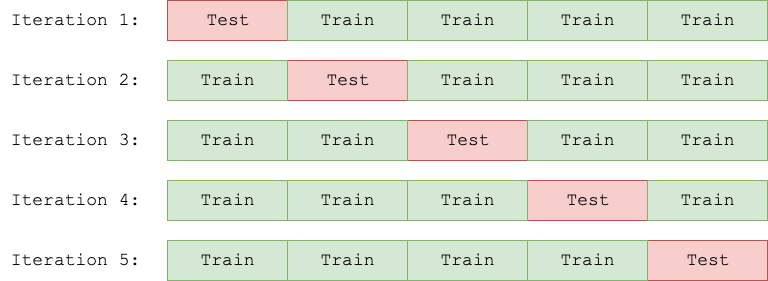
\includegraphics[width=\linewidth]{figures/five_fold_cv.png}
	\caption{Visualisation of a five-fold cross-validation. The data is split into $k=5$ samples, and used exactly once as the validation sample. }
	\label{fig:five_fold_cv}
	\end{center}
\end{figure}

\subsection{Machine learning pipeline}

We used the \textit{scikit-learn} function \texttt{GridSearchCV} to implement a gridsearch coupled with a k-fold cross-validation \cite{scikit-gridsearch}. Our implementation trains a model using every potential combination of parameters, and uses a 5-fold cross validation to identify the best configurations. The value $k=5$ was chosen to give enough samples to allow for generalisation, whilst remaining computationally feasible on the hardware we have available.

Only the best parameter configurations from this process were used for model evaluation. This involved training on all data from 2007 to 2016 and testing on the 2017 data. Each model was evaluated using the coefficient of determination, known as \textit{R-squared} ($R^2$), which gives the proportion of the variance in the dependant variable that is predictable from the independent variable \cite{cameron1997r}. In addition to this, the root mean squared error (RMSE) was used to measure the difference between the values predicted by the model, and the observed values. This pipeline process is visualised in Figure \ref{fig:mlpipeline}.

\begin{figure}[htbp]
	\begin{center}
    	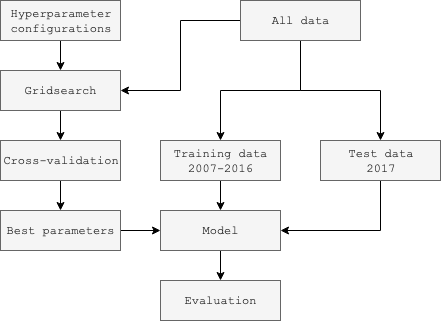
\includegraphics[width=\linewidth]{figures/ml_pipeline.png}
	\caption{Visualisation of the machine learning pipeline. Only the best parameters are used to evaluate the performance of our models. }
	\label{fig:mlpipeline}
	\end{center}
\end{figure}

\subsection{Parameter Optimisation Results}

\begin{figure*}[htbp]
	\begin{center}
    	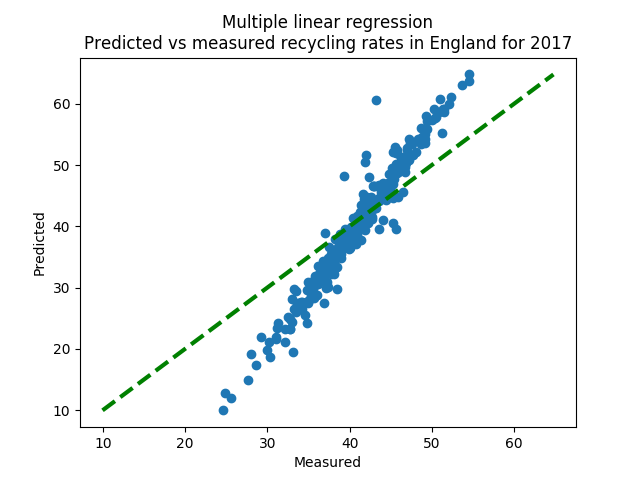
\includegraphics[width=0.32\linewidth]{../figures/england_recycling_predicted_mlr_2017.png}
    	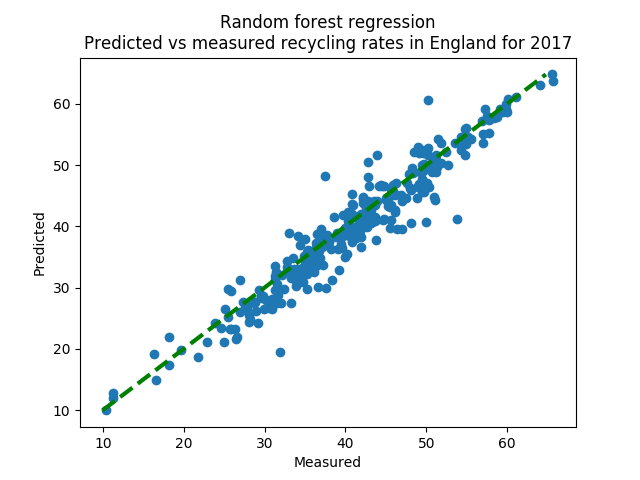
\includegraphics[width=0.32\linewidth]{../figures/england_recycling_predicted_rfm_2017.png}
    	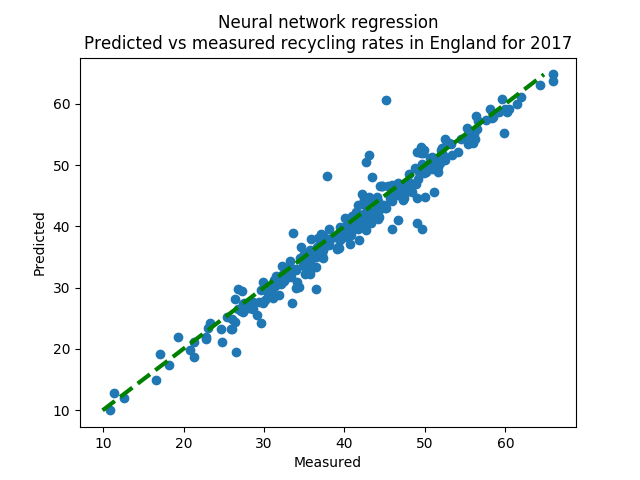
\includegraphics[width=0.32\linewidth]{../figures/england_recycling_predicted_mlp_2017.png}
	\caption{Measured vs predicted values for each local authority in the 2017 data set. A perfect prediction is shown as the green dashed line.}
	\label{fig:predictions}
	\end{center}
\end{figure*}
\subsubsection{Linear Regression}
As multiple linear regression has no real hyperparameters, the default configuration was used for this model.

\subsubsection{Random forest}
We varied three hyperparameters for the random forest model:

\begin{itemize}
\item \textbf{n\_estimators}: The number of decision trees in the ensemble in the range of 5 to 30.
\item \textbf{criterion}: The function to measure the quality of a split. One of: $\{$mean square error, mean absolute error$\}$

\item \textbf{max\_features}: The number of features to consider when looking for the best split. One of:  $\{$n\_features, sqrt(n\_features), log2(n\_features)$\}$
\end{itemize}
The best hyperparameter configuration for the random forest model was using 26 trees, with the mean squared error criterion using the square root of the number of features as the maximum number of features required for a split.

\subsubsection{Neural Network}
Due to the large number of potential configurations, hyperparameter selection is crucial when training a neural network. To enable the machine learning pipeline to be applied to a \texttt{keras} model, it needed to be wrapped in a \texttt{scikit-learn} model wrapper. Using an NVIDIA GeForce 1050 Ti GPU, the hyperparameter selection took 22 hours.

Our parameters were selected from the following set:
\begin{itemize}
    \item \textbf{optimizer}: The function that is applied to the weight parameters to minimise the loss function. One of $\{$ RMSprop, Adagrad, Adadelta, Adam, Adamax, Nadam$\}$
    \item \textbf{activation}: The function that governs the output of a node. One of: $\{$relu, tanh, sigmoid $\}$
    \item \textbf{init\_mode}: The distribution that governs the initial state of the network weights. One of: $\{$uniform, normal $\}$
    \item \textbf{node\_count}: The number of nodes in each layer. One of: $\{$16, 32, 64, 128, 256 $\}$
\end{itemize}

The best parameter configuration for the neural network was using the Adamax optimiser, with 64 nodes per layer using the rectified linear unit activation function (relu), with the weights initialised using a normal distribution. A relu activation function outputs a 0 for any negative value, and returns the input for any positive values \cite{goodfellow2016deep}. 

Figure \ref{fig:nntraining} shows the validation mean error over time, with each time step corresponding to a single training epoch. The validation mean error sharply decreases after the first epoch, then fluctuates throughout the rest of the training run. This indicates that the model fits to the training data quickly, and may not benefit from an extended training time.
\begin{figure}[htbp]
	\begin{center}
    	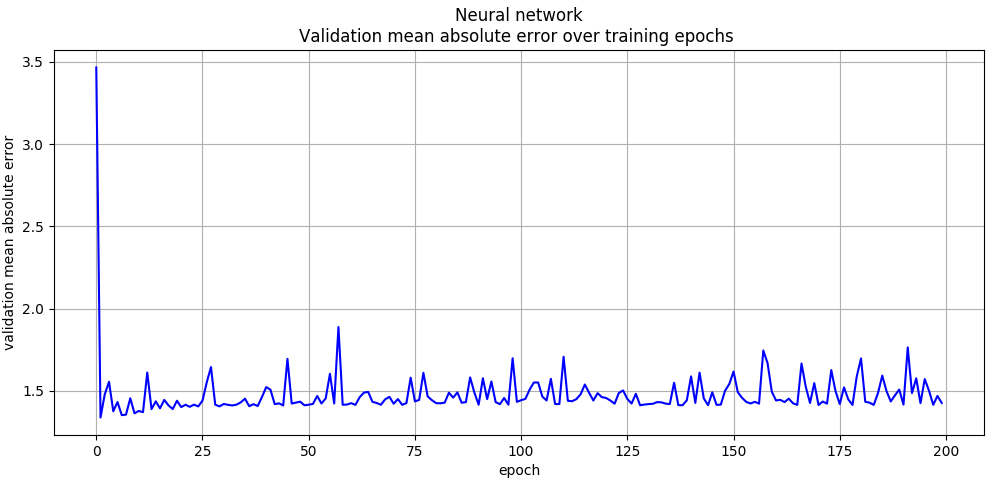
\includegraphics[width=\linewidth]{figures/neural_network_training.png}
	\caption{Training history of the neural network. The validation mean absolute error varies over 200 training epochs. }
	\label{fig:nntraining}
	\end{center}
\end{figure}

\section{Results}

The results of the regression analysis are shown in Table \ref{table:params}. The neural network was the best performing model, achieving a peak $R^2$ value of 0.947 and RMSE of 2.323, when using the population density, index of deprivation, and previous years recycling efficiency as input varaibles. The recycling efficiency of the previous year proved to be the most valuable variable for predicting future recycling efficiency. All other variables when used alone gave worse results overall, and insignificantly improved the RMSE when used in conjunction with previous recycling efficiency, suggesting that they have only a marginal impact at best.  

Interestingly, the random forest model achieved an $R^2$ value of 0.823 when using the index of deprivation as its sole variable. As the index of deprivation is a largely static, we speculate that the random forest model learned the recycling efficiency associated to each local authority, using the index of deprivation as a proxy. This explains why none of the other regression models could learn the relationship.

Figure \ref{fig:predictions} shows a strong positive linear association between the measured and predicted values for all three models, and there appears to be only one outlier. A perfect linear correlation in this figure would mean that all predictions were correct. The multiple linear regression model appears to have learned a tight relationship, however the slope of the $y$-intercept appears to be too small.  Each classifier performs well, which makes it difficult to determine performance by eye. 

Figure \ref{fig:selected_predictions} shows the recycling efficiency of a selection of local authorities over time (in various translucent colours) selected to demonstrate the range of the data. The average value for England is shown in opaque orange. Our predictions for 2017 are marked by an \texttt{x} of the same colour as the corresponding series in the same vertical plane as their actual 2017 values. It is clear that our predictions are close to the true values, however some deviation is to be expected. Given access to the data for 2018, we expect that the same models could be used to predict the recycling efficiency for 2019. 

%\vspace{-0.5cm}
\begin{figure}[htbp]
    \begin{center}
        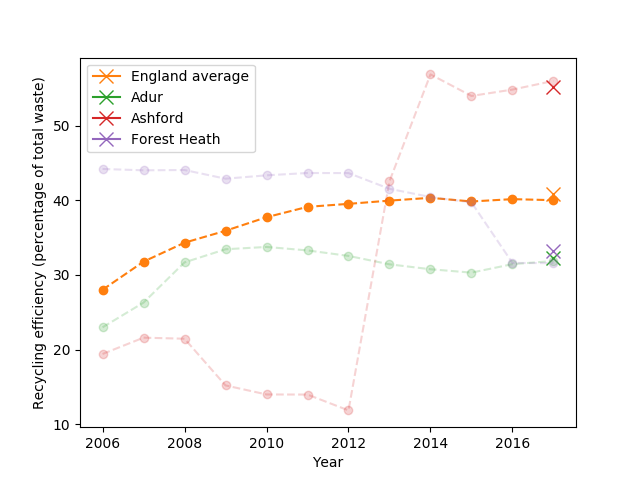
\includegraphics[width=\linewidth]{../figures/england_selected_efficiency_predictions.png}
    \caption{Selected recycling efficiency over time, with predictions made for 2017. All predictions were made using the neural network model and are marked using an \texttt{x}.}
    \label{fig:selected_predictions}
    \end{center}
\end{figure}

%\vspace{-0.5cm}
\section{Conclusions and Future Work}
In general, this work allows us to confirm that we are able to use historical recycling data to make predictions on future recycling efficiency. Other variables such as population density and the index of deprivation may also have an impact. However we have identified that there is no linear or monotonic relationship between these variables and recycling efficiency. Our results are not clear enough to determine that there is no relationship for certain, as there was a marginal improvement when including these in the regression analysis.

Additionally, we found that environmental spending does not have a causal relationship with recycling efficiency, and it is likely that changes to recycling habits are as a result of social factors rather than economic ones. A further investigation could try to gauge public opinion and recycling awareness over time, however we have not been able to find data for such statistics. 

Our results focus solely on the data for domestic recycling, however a large portion of global waste is generated from factories and other commercial facilities. It would be interesting to compare our results with this data, and to see if our pipeline can be generalised to make predictions on the recycling efficiency of manufacturers.

We did not investigate the spatial component of our data. Although we plotted the recycling efficiency of local authorities, we did not perform additional tests to measure if neighbouring authorities have similar recycling rates. Further to this, our work could also be extended to look at the recycling rates of the other countries in the United Kingdom, as well as Europe and the rest of the world. 

The European Union has set a target to recycle 50\% of domestic waste by 2020, however without the data for 2019, our solution is unable to provide an estimate as to whether on not this target will be met. 



\bibliography{bibliography}{}
\bibliographystyle{IEEEtran}
\end{document}

\iffalse
http://lup.lub.lu.se/luur/download?func=downloadFile&recordOId=2365832&fileOId=2365838
https://www.theguardian.com/environment/2018/oct/20/plastic-recycling-industrys-problems-costing-councils-up-to-500000-a-year 
https://scikit-learn.org/stable/modules/cross_validation.html
https://www.gov.uk/government/statistics/english-indices-of-deprivation-2015
https://www.isonomia.co.uk/goodbye-englands-rise-why-have-household-recycling-rates-stalled/
Myers, Jerome L.; Well, Arnold D. (2003). Research Design and Statistical Analysis (2nd ed.). Lawrence Erlbaum. p. 508. ISBN 978-0-8058-4037-7.
https://www.investopedia.com/terms/m/mlr.asp
https://www.recycle-more.co.uk/household-zone/top-facts
https://www.recyclingbins.co.uk/recycling-facts/
https://www.earthday.org/2018/04/05/fact-sheet-plastics-in-the-ocean/
https://www.independent.co.uk/environment/nature/how-scientists-plan-to-clean-up-the-plastic-waste-threatening-marine-life-a6820276.html



Notes:
Go back and check the marking criteria!
Justify all decisions & discussion of available data sets. Why did we choose this data?
There may be confounding variables, eg: population and environmental spending may be related (places with more people spend more on environmental services)
Random forest is best because resilient to zero values
Maybe we use a recurrent architecture for the neural net to account for temporal data? 
Is there a relationship between neighbouring counties? 
Measuring significance through time - lag between budget cut and effect. Bonus points for doing research into methods and thinking about things like this 

\fi
